%\title{Modelo de Projeto de pesquisa}
%% abtex2-modelo-projeto-pesquisa.tex, v-1.9 laurocesar
%% Copyright 2012-2013 by abnTeX2 group at http://abntex2.googlecode.com/ 
%%
%% This work may be distributed and/or modified under the
%% conditions of the LaTeX Project Public License, either version 1.3
%% of this license or (at your option) any later version.
%% The latest version of this license is in
%%   http://www.latex-project.org/lppl.txt
%% and version 1.3 or later is part of all distributions of LaTeX
%% version 2005/12/01 or later.
%%
%% This work has the LPPL maintenance status `maintained'.
%% 
%% The Current Maintainer of this work is the abnTeX2 team, led
%% by Lauro César Araujo. Further information are available on 
%% http://abntex2.googlecode.com/
%%
%% This work consists of the files abntex2-modelo-projeto-pesquisa.tex
%% and abntex2-modelo-references.bib
%%

% ------------------------------------------------------------------------
% ------------------------------------------------------------------------
% abnTeX2: Modelo de Projeto de pesquisa em conformidade com 
% ABNT NBR 15287:2011 Informação e documentação - Projeto de pesquisa -
% Apresentação 
% ------------------------------------------------------------------------ 
% ------------------------------------------------------------------------

\documentclass[
	% -- opções da classe memoir --
	12pt,				% tamanho da fonte
	openright,			% capítulos começam em pág ímpar (insere página vazia caso preciso)
	twoside,			% para impressão em verso e anverso. Oposto a oneside
	a4paper,			% tamanho do papel. 
	% -- opções da classe abntex2 --
	%chapter=TITLE,		% títulos de capítulos convertidos em letras maiúsculas
	%section=TITLE,		% títulos de seções convertidos em letras maiúsculas
	%subsection=TITLE,	% títulos de subseções convertidos em letras maiúsculas
	%subsubsection=TITLE,% títulos de subsubseções convertidos em letras maiúsculas
	% -- opções do pacote babel --
	english,			% idioma adicional para hifenização
	french,				% idioma adicional para hifenização
	spanish,			% idioma adicional para hifenização
	brazil,				% o último idioma é o principal do documento
	]{abntex2}

% ---
% PACOTES
% ---

% ---
% Pacotes fundamentais 
% ---
\usepackage{lmodern}			% Usa a fonte Latin Modern
\usepackage[T1]{fontenc}		% Selecao de codigos de fonte.
\usepackage[utf8]{inputenc}		% Codificacao do documento (conversão automática dos acentos)
\usepackage{indentfirst}		% Indenta o primeiro parágrafo de cada seção.
\usepackage{color}				% Controle das cores
\usepackage{graphicx}			% Inclusão de gráficos
\usepackage{microtype} 			% para melhorias de justificação
\usepackage{subcaption}			% para legenda de imagens
\usepackage{textcomp}
\usepackage{siunitx}


% ---

% ---
% Referência às imagens usadas no projeto:
% ---
\graphicspath{ {img/} }
% ---

% ---
% Caracteres especiais:
% ---
\sisetup{math-micro=\text{µ},text-micro=µ}

% ---
% Pacotes adicionais, usados apenas no âmbito do Modelo Canônico do abnteX2
% ---
\usepackage{lipsum}				% para geração de dummy text
% ---

% ---
% Pacotes de citações
% ---
\usepackage[brazilian,hyperpageref]{backref}	 % Paginas com as citações na bibl
\usepackage[alf]{abntex2cite}	% Citações padrão ABNT

% --- 
% CONFIGURAÇÕES DE PACOTES
% --- 

% ---
% Configurações do pacote backref
% Usado sem a opção hyperpageref de backref
\renewcommand{\backrefpagesname}{Citado na(s) página(s):~}
% Texto padrão antes do número das páginas
\renewcommand{\backref}{}
% Define os textos da citação
\renewcommand*{\backrefalt}[4]{
	\ifcase #1 %
		Nenhuma citação no texto.%
	\or
		Citado na página #2.%
	\else
		Citado #1 vezes nas páginas #2.%
	\fi}%
% ---

% ---
% Informações de dados para CAPA e FOLHA DE ROSTO
% ---
\titulo{Trabalho de conclusão de curso}
\autor{Ceres Rohana e Thaynara Santos}
\local{Brasil}
\data{2017, v-1.0}
\instituicao{%
  Instituto Infnet
  \par
  Faculdade de Engenharia da Computação}
\tipotrabalho{Trabalho de Conclusão de Curso}
% O preambulo deve conter o tipo do trabalho, o objetivo, 
% o nome da instituição e a área de concentração 
\preambulo{Sistema de monitoramento de gases poluentes com o uso de bicicletas}
% ---

% ---
% Configurações de aparência do PDF final

% alterando o aspecto da cor azul
\definecolor{blue}{RGB}{41,5,195}

% informações do PDF
\makeatletter
\hypersetup{
     	%pagebackref=true,
		pdftitle={\@title}, 
		pdfauthor={\@author},
    	pdfsubject={\imprimirpreambulo},
	    pdfcreator={LaTeX with abnTeX2},
		pdfkeywords={abnt}{latex}{abntex}{abntex2}{projeto de pesquisa}, 
		colorlinks=true,       		% false: boxed links; true: colored links
    	linkcolor=blue,          	% color of internal links
    	citecolor=blue,        		% color of links to bibliography
    	filecolor=magenta,      		% color of file links
		urlcolor=blue,
		bookmarksdepth=4
}
\makeatother
% --- 

% --- 
% Espaçamentos entre linhas e parágrafos 
% --- 

% O tamanho do parágrafo é dado por:
\setlength{\parindent}{1.3cm}

% Controle do espaçamento entre um parágrafo e outro:
\setlength{\parskip}{0.2cm}  % tente também \onelineskip

% ---
% compila o indice
% ---
\makeindex
% ---

% ----
% Início do documento
% ----
\begin{document}

% Retira espaço extra obsoleto entre as frases.
\frenchspacing 

% ----------------------------------------------------------
% ELEMENTOS PRÉ-TEXTUAIS
% ----------------------------------------------------------
% \pretextual

% ---
% Capa
% ---
\imprimircapa
% ---

% ---
% Folha de rosto
% ---
\imprimirfolhaderosto
% ---

% ---
% Inserir lista de ilustrações
% ---
% \pdfbookmark[0]{\listfigurename}{lof}
% \listoffigures*
% \cleardoublepage
% ---

% ---
% Inserir lista de tabelas
% ---
% \pdfbookmark[0]{\listtablename}{lot}
% \listoftables*
% \cleardoublepage
% ---

% ---
% Inserir lista de abreviaturas e siglas
% ---
% \begin{siglas}
%   \item[Fig.] Area of the $i^{th}$ component
%   \item[456] Isto é um número
%   \item[123] Isto é outro número
%   \item[lauro cesar] este é o meu nome
% \end{siglas}
% ---

% ---
% Inserir lista de símbolos
% ---
% \begin{simbolos}
%   \item[$ \Gamma $] Letra grega Gama
%   \item[$ \Lambda $] Lambda
%   \item[$ \zeta $] Letra grega minúscula zeta
%   \item[$ \in $] Pertence
% \end{simbolos}
% ---

% ---
% Inserir o sumário
% ---
\pdfbookmark[0]{\contentsname}{toc}
\tableofcontents*
\cleardoublepage
% ---

% ----------------------------------------------------------
% ELEMENTOS TEXTUAIS
% ----------------------------------------------------------
\textual

% ----------------------------------------------------------
% Introdução
% ----------------------------------------------------------
\chapter*[Introdução]{Introdução}
\addcontentsline{toc}{chapter}{Introdução}

% ----------------------------------------------------------
% 1 Introdução
% ----------------------------------------------------------

Em 2015, na sede da ONU de Nova Iorque, aconteceu um encontro entre todos os países das Nações 
Unidas, com o objetivo de traçar metas visando o desenvolvimento sustentável. Com isso, uma agenda 
foi desenvolvida e nomeada de Objetivos de Desenvolvimento Sustentável. 

Dentre os 17 objetivos identificados, o 11º é descrito como \"Tornar as cidades e os assentamentos 
humanos inclusivos, seguros, resilientes e sustentáveis", chamando a atenção para as taxas 
alarmantes de emissão de gases residuais principalmente em áreas urbanas. Em 2015 foi registrado que 
metade da população mundial vive em grandes cidades e a previsão para 2030 é que essa porcentagem 
suba para 60\%, ou seja, as cidades que ocupam aproximadamente apenas 2\% da área do planeta irão 
abrigar 60\% da humanidade, consumindo 80\% da energia produzida e causando 75\% da emissão de gases 
poluentes na atmosfera. 

No Brasil, o crescimento desgovernado nas metrópoles tem ameaçado a infraestrutura não planejada, 
enfatizando problemas como oferta de água potável, esgoto, saúde pública, transporte, qualidade do 
ar, conservação de energia, diminuição do impacto gerado pelo trânsito, dentre outros. Em 2016, 
segundo uma pesquisa implementada pela Organização Mundial da Saúde (OMS), 92\% da população mundial 
esteve exposta a níveis alarmantes de poluição e 7  milhões de pessoas morreram devido à degradação 
ambiental - sendo 4 milhões relacionadas ao uso da madeira, carvão e biomassa, e 3 milhões aos gases 
residuais liberados por veículos automotores. Surpreendentemente, esse número excede a quantidade de 
mortes por síndrome da imunodeficiência adquirida (do termo em inglês: \"Acquired Immunodeficiency 
Syndrome\" - AIDS) e malária juntos.

De acordo com a OMS, os problemas relacionados à exposição constante de poluentes são o AVC 
(Acidente Vascular Cerebral), problemas respiratórios, diabetes, doenças cardiovasculares, câncer e 
infertilidade. Tais problemas podem ser influenciados ou catalisados por compostos orgânicos 
voláteis, como tinta de parede, revestimento de carpete e produtos de limpeza, até os gases 
liberados pelas indústrias e veículos automotores.

Quando gases ou partículas emitidos pela ação humana atingem concentrações suficientemente altas que 
causam danos diretos à população, seja ela humana ou não, um requisito básico para o bem estar de 
todos é negligenciado.

O projeto estadual MonitorAR Rio coleta dados de emissão de gases poluentes desde 2010, nas regiões 
Centro, Copacabana, São Cristóvão, Tijuca, Irajá, Bangu, Campo Grande, Pedra de Guaratiba e Recreio. 
Em 2011 e 2012, os seguintes dados referentes a taxa de gases poluentes coletados foram:

\begin{figure*}
	\centering
	\begin{subfigure}{0.5\textwidth}
		\centering
		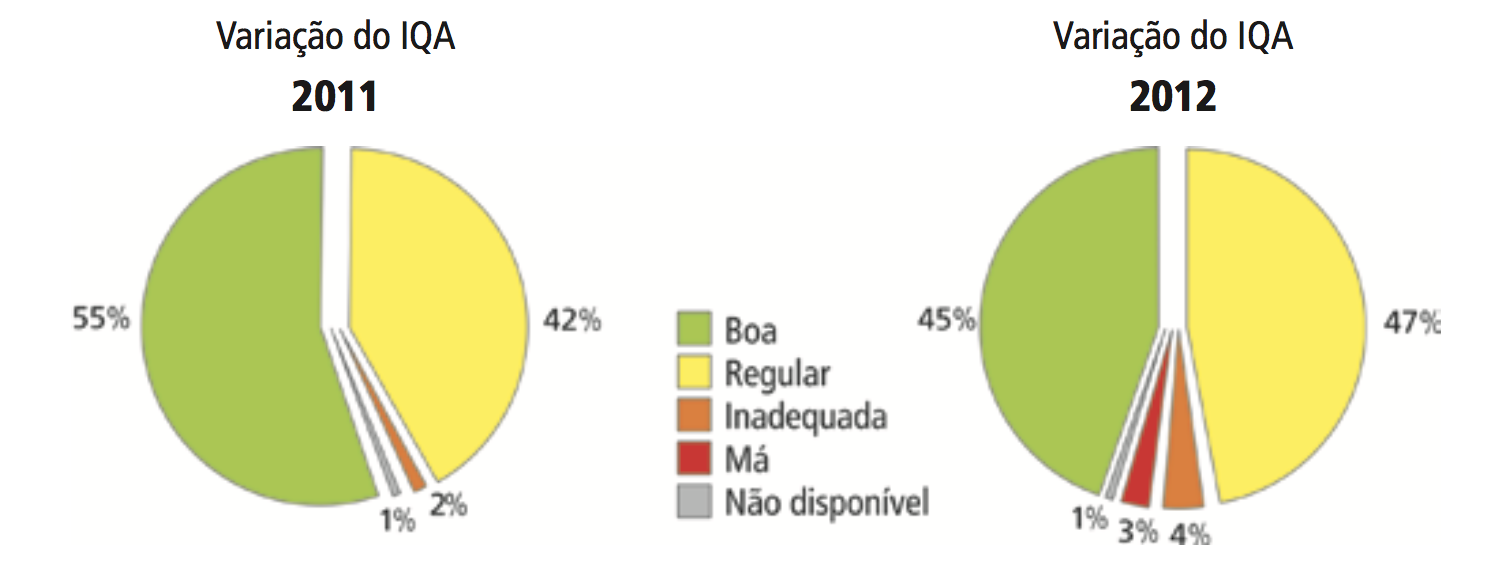
\includegraphics[scale=0.6]{chapter1-img1}
	\end{subfigure}
    \par
    \phantomcaption \small { 
        Gráfico com a variação do IQA 2011: 
        \par
        Bom 55\% | Regular 42\% | Inadequado 2\% | Ruim 0\% | Não disponível 1\% 
        \par
        Fonte: Relatório da Rede MonitorAr-Rio, 2011-2012 }
\end{figure*}

\begin{figure*}
	\centering
	\begin{subfigure}{0.5\textwidth}
		\centering
		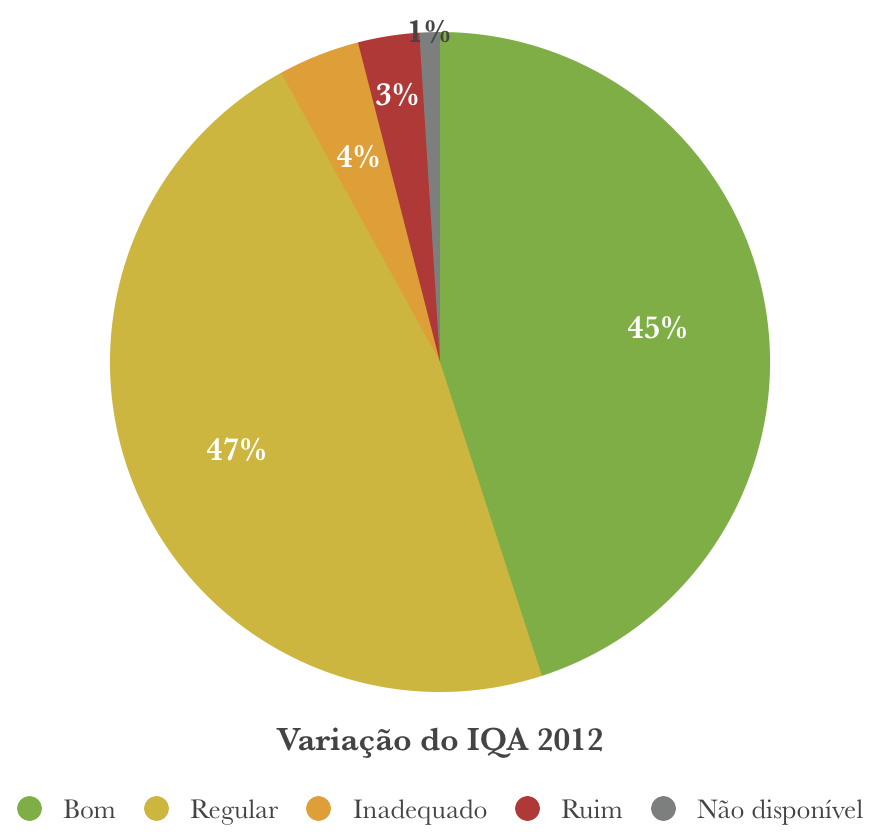
\includegraphics[scale=0.6]{chapter1-img2}
	\end{subfigure}
    \par
    \phantomcaption \small { 
        Gráfico com a variação do IQA 2012: 
        \par
        Bom 45\% | Regular 47\% | Inadequado 4\% | Ruim 3\% | Não disponível 1\%
        \par
        Fonte: Relatório da Rede MonitorAr-Rio, 2011-2012 }
\end{figure*}

\begin{figure*}
	\centering
	\begin{subfigure}{0.5\textwidth}
		\centering
		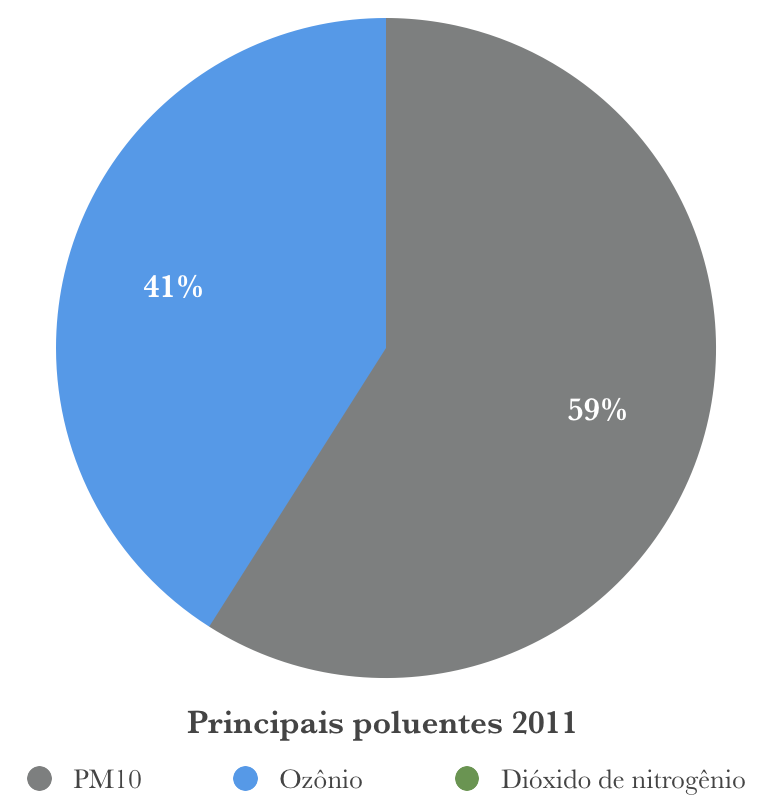
\includegraphics[scale=0.6]{chapter1-img3}
	\end{subfigure}
    \par
    \phantomcaption \small { 
        Gráfico com principais poluentes de 2011: 
        \par
        PM10 59\% | Ozônio 41\% | Dióxido de nitrogênio 0\%
        \par
        Fonte: Relatório da Rede MonitorAr-Rio, 2011-2012 }
\end{figure*}

\begin{figure*}
	\centering
	\begin{subfigure}{0.5\textwidth}
		\centering
		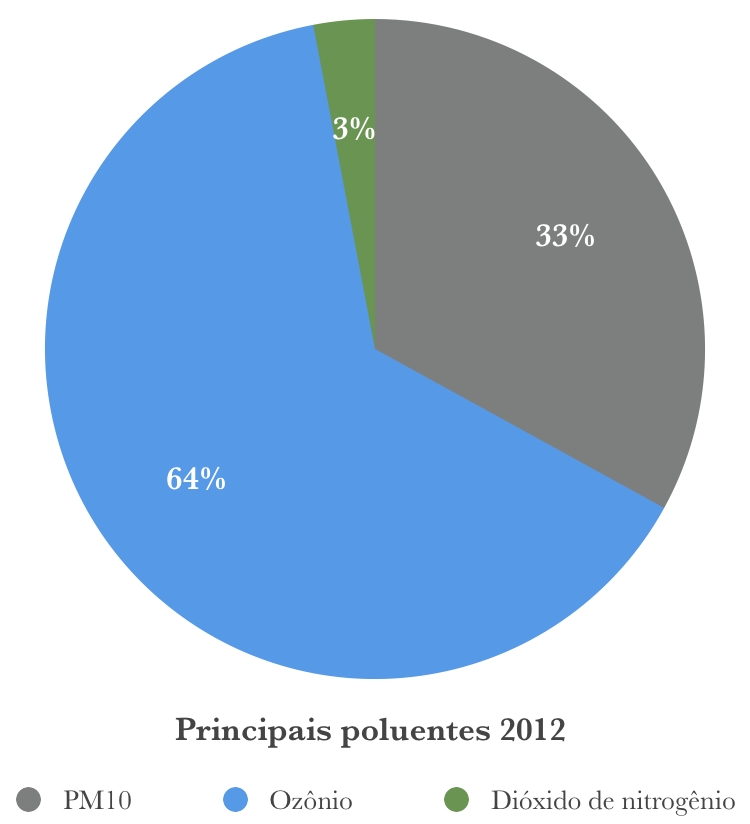
\includegraphics[scale=0.6]{chapter1-img4}
	\end{subfigure}
    \par
    \phantomcaption \small { 
        Gráfico com principais poluentes de 2012:
        \par
        PM10 33\% | Ozônio 64\% | Dióxido de nitrogênio 3\% 
        \par
        Fonte: Relatório da Rede MonitorAr-Rio, 2011-2012 }
\end{figure*}

Dentro dessa perspectiva, voltados para a questão da qualidade do ar e do impacto gerado pelo 
trânsito, urbanistas de todo o mundo se reuniram para discutir e desenvolver programas urbanísticos 
de baixo nível de agressão ambiental, bem como buscar definir um desenvolvimento socioeconômico que 
melhore e não destrua o meio ambiente natural e construído.

Algumas cidades europeias, percebendo a importância de transportes alternativos, priorizaram a 
bicicleta no trânsito, com a intenção de diminuir a poluição ambiental, humanizar as ruas e reduzir 
a quantidade de acidentes. Para isso o governo disponibilizou bicicletas públicas e investiu na 
construção de redes cicloviárias interligadas a outros transportes públicos, como metrô, barcas, 
trens e etc. No Brasil, um exemplo de programa semelhante é o BikeRio. Esse programa foi desenvolvido 
pelo governo do Rio de Janeiro em parceria com o Itaú, promovendo o aluguel de bicicletas por um 
valor mensal ou diário acessível. Ainda que o BikeRio seja um sucesso, o uso da bicicleta ainda 
encontra fortes obstáculos, especialmente por causa da falta de cidadania e respeito no trânsito e 
pelas ciclovias escassas e de má qualidade - mesmo em cidades como Curitiba e Rio de Janeiro, onde 
existe um investimento mais forte nesse contexto.

Além de usada como meio de transporte, a bicicleta é boa para a saúde, sendo considerada uma das 
melhores técnicas para prevenir e tratar a hipertensão, o infarto do miocárdio e o colesterol alto.

Este trabalho tem como objetivo mensurar a quantidade de ar poluído inalado, em média, pelo ciclista 
carioca das regiões urbanas. Um dispositivo embarcado será instalado na bicicleta, com a capacidade 
de captar o nível de gases poluentes durante o trajeto do ciclista. Os dados poderão ser consultados 
em tempo real através de uma página web.

Para alcançar este propósito, será criado um protótipo com o Arduino Trinket, principalmente por ser 
uma placa pequena, de fácil implementação e com diversas portas I/O, flexibilizando a inclusão dos 
sensores. O protótipo será planejado baseado em redes LoRa. Estas são redes sem fio de alto alcance 
e baixo consumo de energia, criadas especificamente para promover a comunicação entre dispositivos 
embarcados (IoT). Com isso, é possível acessar os dados captados por cada usuário em tempo real.

No capítulo 2, \"Resumo histórico e estado da arte", serão apresentadas diversas pesquisas referentes 
ao tema do trabalho, evidenciando as tecnologias e soluções encontradas até o presente momento, para 
mitigar os problemas relacionados; no capítulo 3 - \"Proposição do problema" - o problema, encontrado 
através das pesquisas, será brevemente descrito; e no capítulo 4 - \"Solução proposta" - a solução 
proposta será apresentada, abordando os aspectos tecnológicos e suas premissas, contendo uma visão 
geral do sistema a ser desenvolvido.

% TODO: Quando um novo capítulo for adicionado, adicionar a descrição aqui.

% ----------------------------------------------------------
% Capítulo 1: Breve resumo histórico
% ----------------------------------------------------------
\chapter{Breve resumo histórico}

% ----------------------------------------------------------
% Capítulo 1: Breve resumo histórico
% ----------------------------------------------------------

\section{Pesquisas de medição da poluição}

Segundo a pesquisa (GOUVEIA, Nelson, 2017) a poluição do ar é uma importante preocupação de saúde 
pública, especialmente para crianças particularmente suscetíveis. A América Latina tem uma grande 
população infantil, é altamente urbanizada e os níveis de poluição são substancialmente altos, o que 
agrava o impacto potencial da poluição atmosférica na saúde. Portanto, foi analisado o efeito da 
poluição do ar sobre a mortalidade respiratória infantil em quatro grandes centros urbanos: Cidade 
do México, Santiago no Chile, São Paulo e Rio de Janeiro no Brasil.

O estudo realizou uma análise estatística dos índices de mortalidade por doenças respiratórias em 
lactentes e crianças, em relação aos níveis de PM10 - partículas inaláveis, de diâmetro inferior a 
10 micrometros (\SI{10}{ \micro\meter }) e O\textsubscript{3} (ozônio), analisando os efeitos conforme faixa etária e 
cidade. 

Foram demonstradas estimativas de mortalidade, em relação ao impacto dos poluentes atmosféricos em 
todas essas cidades e grupos etários. Esta informação é importante, pois muitas políticas públicas 
destinadas a prevenir os efeitos adversos da poluição na saúde consideram as crianças como o grupo 
populacional que merece a maior proteção.

Essas cidades receberam quase 43 milhões de pessoas e os níveis de poluição estavam acima das 
diretrizes da OMS. Para PM10, o aumento percentual do risco de morte, devido as doenças 
respiratórias, em lactentes em um modelo de efeito fixo foi de 0,47\%. Para as mortes respiratórias 
em crianças de 1 a 5 anos, o aumento de risco foi de 0,58\%, observando-se maior efeito nas 
infecções respiratórias inferiores (do termo em inglês: ``low respiratory infections'' - LRI) em 
crianças de 1 a 14 anos, sendo de 1,38\%. Para O\textsubscript{3}, a única estimativa resumida 
estatisticamente significante foi para LRI em lactentes. A análise por temporada mostrou efeitos de 
O\textsubscript{3} no verão para doenças respiratórias em lactentes, enquanto os efeitos negativos 
foram observados para as mortes respiratórias e LRI em crianças.

De acordo com o estudo realizado para localizar pontos de concentração de carbono preto e PM2.5 em 
áreas urbanas (TARGINO, Admir C., 2016), foram utilizadas três bicicletas instrumentadas foram 
usadas para medir as concentrações de carbono preto (do termo em inglês: ``Black Carbon'' - BC) e 
PM2.5 - partículas inaláveis, de diâmetro inferior a 2.5 micrometros (\SI{3}{ \micro\meter }), em 
uma cidade de médio porte no sul do Brasil. O objetivo deste estudo foi mapear a distribuição 
espacial de BC e PM2.5, identificar as localidades de maior concentração de poluição do ar e avaliar 
fatores que possam afetar as concentrações desses poluentes, por exemplo, volume de tráfego, número 
de veículos diesel pesados (do termo em inglês: ``Heavy-duty diesel vehicles'' - HDDV), posição dos 
sinais de trânsito e inclinação da rua. 

Os ciclistas coletaram dados no centro da cidade ao longo de ruas de diferentes densidades de 
tráfego durante nove sessões de amostragem, nos períodos da manhã e da tarde, entre 13 de março e 28 
de abril de 2015. A amostragem em bicicleta abrangeu uma área de 
\SI{2.7}{ \kilo\meter\textsuperscript{2} }, sobre elevação variável, e percorreu uma distância total 
de \SI{215}{ \kilo\meter\ }. O carbono preto e o PM2.5 exibiram uma grande variabilidade espacial em 
uma escala de dezenas de metros, e as concentrações foram positivamente correlacionadas com as 
contagens de tráfego, mas apresentaram uma relação mais forte com o número de veículos diesel pesados. 

Esses resultados implicam que ônibus antigos e caminhões diesel podem ser os principais agentes dos 
altos níveis de poluição no núcleo interno da cidade. Portando, foi observada uma forte relação 
entre as concentrações de carbono preto nas junções geridas pelos sinais de trânsito e a quantidade 
de HDDV. A concentração média de carbono preto foi de \SI{8.10}{ \micro\meter } perto de sinais de 
trânsito localizados em uma rua inclinada (com mais de 100 veículos movidos a diesel) em comparação 
com sinais de trânsito em terreno plano, que foi de \SI{6}{ \micro\meter }, o que pode ser atribuído 
a maior aceleração necessária no início do movimento. Esse padrão foi menos evidente para as 
concentrações de PM2.5.

Em 2016, um estudo foi feito para investigar a dispersão de poluentes em um túnel rodoviário na 
presença de veículo em movimento (BHAUTMAGE, Utkarsh, 2016), por uma abordagem de velocidade relativa 
usando CFD 3-D (Dinâmica de fluido computacional de 3 dimensões). 

O comportamento turbulento do fluxo de ar em torno de veículos de diferentes formas e seu impacto na 
dispersão de poluentes foram estudados. As geometrias do veículo de diferentes formas foram extraídas 
e simplificadas e dimensionadas com base nos veículos típicos nas estradas indianas. O modelo foi 
verificado com os dados da leitura de pressão estática em torno de um corpo de veículo em movimento 
antes de se aplicar para simular concentrações, e ser validado com dados no local.

Os resultados mostraram que as variações na dispersão dos poluentes eram proporcionais ao tamanho, à 
forma e à velocidade dos veículos. O fluxo de tráfego produziu uma dispersão mais alta de poluentes 
e acelerou o efeito do pistão, empurrando poluentes para o túnel e fora do portal de saída em curto 
prazo. As descobertas têm um significado particular nos estudos relacionados à dispersão dentro dos 
túneis com um tráfego misto de diferentes dimensões e formas.

\section{Uso de transporte alternativo}

Os transportes públicos, como trem elétrico, metrô, VLT (Veículo Leve sobre Trilhos) têm um papel 
importante na sustentabilidade e preservação do meio ambiente, pois diminuem a quantidade de 
automóveis, grandes emissores de poluentes nas ruas, e deslocam maior número de pessoas em menor 
período de tempo, por longas distâncias. Além do mais, estas modalidades de transporte de massa podem 
empregar fontes de energia renováveis, como no caso do Brasil, principalmente a energia hidrelétrica. 

Além do transporte público, as bicicletas têm ganhado cada vez mais importância  como meio de 
transporte alternativo. Em alguns países como Índia, Noruega, Colômbia, Alemanha, Austrália, 
Dinamarca, França, China, Espanha e Holanda, a prática da utilização das bicicletas é amplamente 
estimulada pela população. Particularmente, em países como Holanda, considerada capital mundial da 
bicicleta, e Dinamarca, o uso de bicicletas recebe grandes investimentos, em infraestrutura 
cicloviária, educação, sendo considerados também os países mais seguros para os ciclistas.

No Brasil, mais especificamente no Rio de Janeiro, o programa Rio - Estado da Bicicleta tem como 
objetivo incentivar o uso da bicicleta como meio de transporte nas cidades, criado pela Secretaria de 
Transportes do Estado do Rio de Janeiro, que busca promover a integração deste com os outros meios de 
transporte, como trens, metrôs e barcas, ao também disponibilizar bicicletários nas estações; 
elaborar projetos e fomentar a implantação de infraestrutura cicloviária; implantar, em parceria com 
órgãos públicos e privados, políticas e campanhas educacionais; além de promover e apoiar eventos 
esportivos, culturais e institucionais.

\section{Contexto que originou o problema}

Em relação à poluição do ar, as pesquisas comprovaram que ciclistas são mais suscetíveis a inalar 
maiores doses de NO\textsubscript{2} (dióxido de nitrogênio), mas ainda existem outros tipos de 
substâncias que devem ter seus impactos analisados, portanto, com o aumento dos ciclistas, mais 
pessoas podem ser expostas sem ter como base o risco em relação a este fato, por outra via as mesmas 
poderão ser os principais agentes para obtenção dos dados e mudança do quadro.


\section{Estado da arte}

O estado da arte é um momento importante do documento, pois mostra as pesquisas mais recentes e 
relevantes que foram desenvolvidas, no qual é apresentado um ponto de partida para o projeto. Logo, 
iremos apresentar o contexto, através de artigos e pesquisas relacionados ao tema proposto e as 
tecnologias utilizadas atualmente:

De acordo com o estudo (GATELY, Conor, 2017), as emissões na estrada variam amplamente em escalas de 
tempo tão baixas como minutos e escalas de comprimento tão baixas quanto dezenas de metros. Os dados 
detalhados sobre as emissões a essas escalas são um pré-requisito para quantificar com precisão as 
concentrações de poluição ambiental e identificar localidades de maior concentração de exposição 
humana em áreas urbanas.

Para isso, foi construído um inventário altamente resolvido de fluxos crescentes de CO (monóxido de 
carbono), NO\textsubscript{2} (dióxido de nitrogénio), óxidos de nitrogênio, PM2.5 - partículas 
inaláveis, de diâmetro inferior a 2.5 micrómetros (µm), e CO\textsubscript{2} (dióxido de carbono) 
de veículos rodoviários em 280.000 segmentos rodoviários no leste de Massachusetts para o ano de 
2012. O inventário integra um grande banco de dados de informações sobre as velocidades do veículo 
derivadas do celular e dados do GPS, com vários conjuntos de dados regionais de fluxos de veículos, 
características da frota e meteorologia local. Foram quantificadas as emissões de ``excesso'' do 
congestionamento do tráfego, encontrando um aumento modesto do congestionamento (3 à 6\%) em escalas 
regionais, mas centenas de pontos locais com emissões anuais altamente elevadas (até 75\% para 
estradas individuais em pontos extratégicos). As reduções impulsionadas pelo congestionamento na 
economia de combustível do veículo exigiram um consumo excessivo de 113 milhões de galões de 
combustível para motores, no valor de U\$ 415 milhões, mas isso representou apenas 3,5\% do 
combustível total consumido em Massachusetts, já que mais de 80\% da viagem do veículo ocorre em 
condições não verificadas. No domínio de estudo apresentado, as emissões são altamente concentradas 
espacialmente, com 70\% de poluição originária de apenas 10\% das estradas. 

O Inventário Nacional de Emissões (NEI) da EPA de 2011 entende as emissões agregadas de óxidos de 
nitrogênio, PM2.5 e CO\textsubscript{2} em 46\%, 38\% e 18\%, respectivamente. No entanto, as 
emissões de CO permanecem em 5\% para os dois inventários, sugerindo que os grandes preconceitos nas 
emissões de óxidos de nitrogênio e PM2.5 resultam de diferenças nas estimativas da atividade do 
veículo a diesel. Ao fornecer informações detalhadas sobre localidades de maior concentração de 
emissões locais e padrões de emissões regionais, a estrutura do inventário é compatível com 
intervenções de tráfego direcionadas, processo de comparação de produtos mais transparente e 
melhorias na qualidade global do ar urbano.

Segundo o estudo (MCKERCHER, Grant R., 2017), as abordagens tradicionais para medir a qualidade do ar 
com base em medidas fixas são inadequadas para o monitoramento da exposição pessoal. Para combater 
esta questão, o uso de tecnologias pequenas e portáteis de monitoramento da poluição atmosférica está 
aumentando, com pesquisadores e indivíduos que utilizam métodos móveis e portáteis para obter dados 
de poluição atmosférica mais espaciais e temporariamente representativos. No entanto, muitas opções 
comercialmente disponíveis são criadas para várias aplicações e baseadas em diferentes tecnologias, 
pressupostos e limitações. Não existe uma revisão das características de monitoramento de gases na 
literatura científica atual.

Uma revisão de última geração de monitores portáteis que medem poluentes ao ar foi desenvolvida para 
abordar as tendências amplas nos últimos 5 a 10 anos, e para ajudar futuros pesquisadores 
interessados em estudar poluentes atmosféricos, a escolher monitores apropriados para suas 
necessidades de aplicação e amostragem.

As tendências das utilizações de dispositivos pequenos e portáteis para monitoração da poluição do ar 
foram identificadas e discutidas em uma revisão da literatura. Em seguida, pesquisas de bancos de 
dados online foram realizadas para artigos contendo informações específicas relacionadas ao 
desempenho, características e uso de tais monitores que medem um ou mais dos três poluentes 
atmosféricos: ozônio, dióxido de nitrogênio e monóxido de carbono. Todos os dados foram resumidos em 
tabelas de referência para comparação entre aplicativos, recursos físicos, capacidades de detecção e 
custos dos dispositivos.

As recentes tendências de monitoramento portátil estão fortemente relacionadas aos aplicativos e 
públicos associados. A pesquisa fundamental requer monitores com o melhor desempenho individual e, 
portanto, a tecnologia de custo mais alto, ainda que uma colaboração coletiva, permita componentes 
de baixo custo.

Muitos estudos, como (LONGLEY, Ian, 2016), compararam a exposição dos ciclistas àqueles que utilizam 
outros meios de transporte e compararam as diferenças de exposição entre rotas e estradas principais. 

Neste estudo, foi empregado o uso de três bicicletas que viajam em uníssono para amostrar 
concentrações de partículas ultrafinas (UFP), monóxido de carbono (CO) e partículas finas (PM1.0 - 
partículas inaláveis, de diâmetro inferior a 1.0 micrómetro (\SI{1}{ \micro\meter })) a três 
distâncias diferentes do fluxo de tráfego, em uma área central do parque da cidade de Christchurch, 
Nova Zelândia. Pesquisas similares foram feitas usando equipamentos estacionários, mas isso pode não 
representar com precisão as diferenças de exposição ao se mover com um fluxo de veículos. Três 
ciclistas estavam equipados com um conjunto de instrumentos idênticos e pedalando em uma velocidade 
contínua, porém em distâncias diferentes da rua principal. Eles se dividiram entre a calçada da 
estrada (a 7 metros da rua principal) e um caminho fora da estrada (19 metros da rua principal), 
durante um total de 6 horas e 45 minutos, durante o outono. 

Os dados foram analisados sob a forma de modelos lineares mistos, com a posição do ciclista 
(distância da borda da faixa de tráfego mais próxima), velocidade do vento e temperatura, tendo 
efeitos estatisticamente significativos nas exposições médias (p < 0.05). A exposição média às UFP e 
ao CO foi aproximadamente 20 à 30\% (p < 0,01) mais baixa na calçada e 40 à 50\% menor no caminho, 
do que na estrada (p < 0,01). Esses resultados destacam os benefícios da segragação de rua e 
ciclovia, já que poderia ajudar a reduzir a inalação de poluentes pelos ciclistas, especialmente em 
estradas com grande tráfego.

\section{Planejamento de rota de viagem para sistemas de compartilhamento de bicicletas (Novembro 
2016)}

Os sistemas de compartilhamento de bicicletas (do termo em inglês: ``Bicycle-Sharing Systems'' - BSS) 
que oferecem usos de bicicletas compartilhadas ao público estão se tornando cada vez mais populares 
hoje em dia. Nestes sistemas, as pessoas podem emprestar e devolver bicicletas em qualquer estação 
de bicicleta na região do serviço, mas o tempo de viagem livre geralmente é limitado. Portanto, para 
viagens de bicicleta de longa distância, os indivíduos precisam pré-agendar a rota de viagem de 
bicicleta com antecedência e mudar a bicicleta dentro do tempo de viagem livre, de modo que não sejam 
cobradas taxas de horas extras. 

Neste artigo, foi estudado o problema do planejamento da rota de viagem para os indivíduos ao usar os 
sistemas de compartilhamento de bicicletas. Dada a origem e o destino da viagem, foi necessário 
identificar a rota de viagem ideal desde a origem até o destino através das estações de bicicleta. 
Para resolver o problema, foi realizada uma análise minuciosa sobre um BSS existente, Divvy, lançado 
em Chicago. 

Com base nos resultados da análise, uma nova estrutura de planejamento de rotas de bicicleta (do 
termo em inglês: ``BSSs Based Trip Route Planning'' - STOP) foi proposta para identificar a rota de 
viagem ideal, mapeando o problema em um problema de fluxo de rede de custo mínimo. Experimentos 
extensivos realizados em conjuntos de dados do sistema de compartilhamento de bicicleta do mundo 
real demonstram a eficácia do STOP.

Seundo a pesquisa (AUGUSTIN, Aloÿs, 2016), LoRa é um sistema de telecomunicações de longo alcance e 
de baixa potência para a ``Internet das coisas''. A camada física usa a modulação LoRa, uma tecnologia 
proprietária com um protocolo de controle de acesso ao meio (do termo em inglês: ``Media Access 
Control'' - MAC). LoRaWAN é um padrão aberto com a especificação disponível gratuitamente.

Este artigo fornece uma análise abrangente da modulação LoRa, incluindo a taxa de dados, formato do 
quadro, fator de espalhamento, sensibilidade do receptor, etc. Um banco de provas foi construído, 
experimentalmente para estudar o desempenho da rede, documentado neste artigo. 

Os resultados mostraram que a modulação LoRa, graças à modificação do espectro espalhado de chirp e 
alta sensibilidade do receptor, oferece boa resistência à interferência. Testes de campo mostraram 
que a LoRa pode oferecer cobertura de rede satisfatória de até 3 km em uma área suburbana com 
moradias residenciais densas. O fator de espalhamento tem um impacto significativo na cobertura de 
rede, assim como a taxa de dados. A LoRa é, portanto, bem adequada para baixa potência, sistemas não 
críticos e redes de longo alcance. Este artigo também mostrou que a LoRaWAN tem um protocolo LPWAN 
muito semelhante ao ALOHA. Seu desempenho, portanto, se degrada rapidamente quando a carga no link 
aumenta.

Conforme o estudo (BECKX, Carolien, 2016), a exposição à poluição do ar pode ter graves impactos na 
saúde, especialmente para os idosos. Para estimar a dose inalada de poluição do ar, tradicionalmente 
apenas a concentração de poluição do ar no local de residência é considerada, sem incorporar 
comportamento de viagem individual e atividade física. Isso pode levar a um viés na avaliação do 
impacto da saúde e nos estudos epidemiológicos, possivelmente subestimando a exposição à poluição do 
ar e desinformando os formuladores de opiniões. 

O estudo abordou esta questão usando dados precisos do sistema de poscicionamento global (do termo 
em inglês: ``Global Position System'' -  GPS) e acelerômetro de 7 dias em 180 participantes com idade 
entre 58 e 65 anos que vivem em Ghent (Bélgica). A concentração de NO\textsubscript{2} (dióxido de 
nitrogénio) para a Bélgica está disponível a partir de um modelo de regressão do uso da terra. São 
utilizados três métodos para calcular a dose inalada de NO\textsubscript{2}. O primeiro método é o 
método estático tradicional, usando apenas a concentração de NO\textsubscript{2} na localização 
inicial. O segundo método incorpora comportamento de viagem usando dados de GPS, observando assim a 
concentração de NO\textsubscript{2} na localização exata do participante. O terceiro método incorpora 
adicionalmente os dados do acelerômetro e estima o modo de transporte utilizado e a atividade física 
para calcular a taxa de ventilação. Ao incorporar a localização geográfica, as diferenças na dose 
inalada de NO\textsubscript{2} dependem da concentração de NO\textsubscript{2} no local de origem e 
do comportamento de viagem individual. Ao incorporar adicionalmente a taxa de ventilação, a dose 
inalada de NO\textsubscript{2} aumenta em mais de 12\%. Além de comparar estes três métodos entre si, 
a influência do modo de transporte é testada. 

O ciclismo está associado ao aumento das doses inaladas de NO\textsubscript{2} em relação aos outros 
meios de transporte. O NO\textsubscript{2} é um gás irritante para os pulmões e diminui a resistência 
às infecções respiratórias. Os efeitos às exposições de curto prazo ainda não são bem conhecidos, 
mas a exposição frequente a níveis relativamente elevados pode provocar tendência para problemas 
respiratórios em crianças e grupos de risco como os asmáticos.

Além de fatores, como faixa etária, região e alimentação, que são sempre levados em consideração em 
experimentos, também é importante levar em consideração as atividades físicas de cada indivíduo, pois 
as mesmas também influenciam nas doses de substâncias inaladas, e conforme o estudo, isso pode ser 
feito com precisão através do GPS e acelerômetro.

De acordo com os artigos apresentados, podemos verificar que até o presente momento pesquisas foram 
realizadas para encontrar os níveis de poluição as quais os seres humanos são expostos, levando em 
consideração os tipos de poluentes do ar, localização geográfica, faixa etária e atividades físicas 
dos indivíduos. Isso foi possível através de redes sem fio, sensores ambientais, GPS e acelerômetros, 
muitas vezes encontrados em celulares e veículos. Além disso as informações geradas e transmitidas a 
longas distâncias também auxiliaram na realização de análises, onde foi possível verificar, através 
de métodos de regressão linear e grafos, as possibilidades de melhoria na urbanização, qualidade do 
ar em determinadas regiões, planejamento de rotas em tempo real e redução de gastos com taxas extras 
em sistemas de compartilhamento de bicicletas.


% ----------------------------------------------------------
% Capitulo de textual  
% ----------------------------------------------------------
\chapter{Elementos textuais}

\index{elementos textuais}A norma ABNT NBR 15287:2011, p. 5, apresenta a
seguinte orientação quanto aos elementos textuais:

\begin{citacao}
O texto deve ser constituído de uma parte introdutória, na qual devem ser
expostos o tema do projeto, o problema a ser abordado, a(s) hipótese(s),
quando couber(em), bem como o(s) objetivo(s) a ser(em) atingido(s) e a(s)
justificativa(s). É necessário que sejam indicados o referencial teórico que
o embasa, a metodologia a ser utilizada, assim como os recursos e o cronograma
necessários à sua consecução.
\end{citacao}

Consulte as demais normas da série ``Informação e documentação'' da ABNT
para outras informações. Uma lista com as principais normas dessa série, todas
observadas pelo \abnTeX, é apresentada em \citeonline{abntex2classe}.

% ----------------------------------------------------------
% Capitulo com exemplos de comandos inseridos de arquivo externo 
% ----------------------------------------------------------

\include{abntex2-modelo-include-comandos}

% ---
% Finaliza a parte no bookmark do PDF
% para que se inicie o bookmark na raiz
% e adiciona espaço de parte no Sumário
% ---
\phantompart

% ---
% Conclusão
% ---
\chapter*[Considerações finais]{Considerações finais}
\addcontentsline{toc}{chapter}{Considerações finais}

\lipsum[31-33]

% ----------------------------------------------------------
% ELEMENTOS PÓS-TEXTUAIS
% ----------------------------------------------------------
\postextual

% ----------------------------------------------------------
% Referências bibliográficas
% ----------------------------------------------------------
\bibliography{abntex2-modelo-references}

% ----------------------------------------------------------
% Glossário
% ----------------------------------------------------------
%
% Consulte o manual da classe abntex2 para orientações sobre o glossário.
%
%\glossary

% ----------------------------------------------------------
% Apêndices
% ----------------------------------------------------------

% ---
% Inicia os apêndices
% ---
\begin{apendicesenv}

% Imprime uma página indicando o início dos apêndices
\partapendices

% ----------------------------------------------------------
\chapter{Quisque libero justo}
% ----------------------------------------------------------

\lipsum[50]

% ----------------------------------------------------------
\chapter{Nullam elementum urna vel imperdiet sodales elit ipsum pharetra ligula
ac pretium ante justo a nulla curabitur tristique arcu eu metus}
% ----------------------------------------------------------
\lipsum[55-57]

\end{apendicesenv}
% ---


% ----------------------------------------------------------
% Anexos
% ----------------------------------------------------------

% ---
% Inicia os anexos
% ---
\begin{anexosenv}

% Imprime uma página indicando o início dos anexos
\partanexos

% ---
\chapter{Morbi ultrices rutrum lorem.}
% ---
\lipsum[30]

% ---
\chapter{Cras non urna sed feugiat cum sociis natoque penatibus et magnis dis
parturient montes nascetur ridiculus mus}
% ---

\lipsum[31]

% ---
\chapter{Fusce facilisis lacinia dui}
% ---

\lipsum[32]

\end{anexosenv}

%---------------------------------------------------------------------
% INDICE REMISSIVO
%---------------------------------------------------------------------

\phantompart

\printindex


\end{document}
